\documentclass[twocolumn,onesided,9pt]{article}

\usepackage{./Task32FlyerLatexStyle/Task32Flyer}
\usepackage{todonotes}

% call all of the roadmap-specific styling
\newcounter{roadmap}

\newtcolorbox[use counter=roadmap, list inside=roadmap,]{roadmap}[2][]{float=htb,
        before={\noindent},
		halign=flush left,
		title={Roadmap \thetcbcounter: #2},
		list text = {#2},
		coltitle=white,
		% fonttitle=\bfseries,
		coltext = TextGrey,
		title filled = true,
		halign title=flush center,
		toptitle=3pt,
		bottomtitle = 3pt,
		every float=\centering,
		width=1.0\columnwidth,
		boxsep=0pt,
		left=3pt,
		right=3pt,
		top=3pt,
		colback=Task32Blue!10!white,
		colframe=Task32Blue,
		subtitle style = {colback=Task32Blue!10!white,
		        colframe=Task32Blue!10!white,
		        fontupper = \bfseries,
		        boxrule = 0pt,
				frame hidden,
				coltitle = TextGrey},
		#1}

\newcommand{\event}[3]{
	% #1 is the over-title
	% #2 is the heading
	% #3 is the explanatory text
	\ifthenelse{\equal{#1}{}}{}{\textbf{#1:}\ }
	{#2}
	\ifthenelse{\equal{#3}{}}{\ignorespaces}{\par\emph{#3}}
}

\newcommand{\taskevent}[5]{
	% #1 is the year
	% #2 is the month, quarter, whatever
	% #3 is the over-title
	% #4 is the heading
	% #5 is the explanatory text
	#1 & #2 & \event{#3}{#4}{#5}
}

\newcommand{\otherevent}[3]{
	% #1 is the year
	% #2 is the month, quarter, whatever
	% #3 is the explanatory text
	\emph{{\color{TextGrey!50!white}#1}} & \emph{{\color{TextGrey!50!white}#2}} & \emph{{\color{TextGrey!50!white}#3}}
}

\newcommand{\rmsubtitle}[2]{%
    \tcbsubtitle{{\color{TextGrey}#1}}
	#2
}

% make some structure
\newcommand{\RMactivities}{%
    \rmsubtitle{Activities}
    }%

% Make a table for old activities
\newenvironment{RMold}%
{% before
\begin{tabular}{@{}p{0.075\columnwidth} p{0.075\columnwidth} p{0.7\columnwidth}@{}}
}
{% after
\end{tabular}
}

% new activities
\newenvironment{RMnew}%
{% before
\begin{tabular}{@{}p{0.075\columnwidth} p{0.075\columnwidth} p{0.7\columnwidth}@{}}
}
{% after
\end{tabular}
}

\addto\captionsenglish{\renewcommand{\figurename}{Roadmap}}

% stop floats slipping too far
\usepackage[section]{placeins}

% add an external link icon
\usepackage[fixed]{fontawesome5}
\newcommand{\extlink}[1]{%
\mbox{\href{#1}{{\small\faExternalLink*}}}%
}



%% -----------------------------------
%% Document information
%% -----------------------------------
\def\pubdate{15 September 2020}
\title{IEA Wind Task 32: Collaborative R\&D Roadmap}
\shorttitle{Collaborative R\&D Roadmap}
\DOI{10.5281/zenodo.4030701}
\addbibresource{bibliography.bib}

%% ===================================
%% Document starts
%% ===================================
\begin{document}

%% -----------------------------------
%% Title
%% -----------------------------------
\maketitle
\thispagestyle{cover}

%% -----------------------------------
%% Introductory text
%% -----------------------------------
{\Large\noindent%
	Task 32 has created a worldwide network of wind lidar researchers who meet regularly to identify opportunities for the use of wind lidar, and mitigate the barriers to its adoption.
}
\vskip 6pt

Wind lidar has many applications for wind energy that span all technology readiness levels. Task 32 connects many stakeholders including the research community, vendors, service providers, and end users with the aim of creating an active network for the exchange of information and experience.

%% -----------------------------------
%% About
%% -----------------------------------
\section*{About IEA Wind Task 32}

\subsection*{Task 32's mission}
Task 32 provides a platform for experts worldwide to collaborate on wind lidar. Together, we identify and mitigate the barriers to adoption of wind lidar for wind energy. We do this by collecting evidence, establishing consensus, and working towards actionable results.

\subsection*{Our vision for wind lidar}
Our members want to see wind lidar as a trusted tool for use in many different wind energy applications.

\subsection*{Get involved}
IEA Wind Task 32 is an international collaboration. It is typically funded on a national level so that many different organisations from a country can take part, leveraging their own resources. Details can be found on the \href{https://community.ieawind.org/task32/about/participants}{Task 32 website}.

As a result of this, we welcome anyone with an interest in wind lidar for wind energy applications to get involved in the Task's activities. This can mean attending our events, contributing to working groups, or helping lead our activities. \textbf{We would very much welcome your help!} \href{https://community.ieawind.org/task32/about/contact}{Contact the Task 32 Operating Agent} to find out more.

\newpage

\section*{About this document}
This document provides an overview of our members' goals and the activities that we have already undertaken, and our plans for the future. They are intended to help stakeholders engage with the Task, provide feedback, and suggest new activities. Although it has been written by the Task Operating Agents and members of the advisory board, \textbf{this roadmap is driven by our members}.

The technical background to these activities is provided in an article written by the Task 32 Advisory Board in 2018 \cite{Clifton_2018_a} and in references cited in the text.

We plan to update this document annually.

\begin{tcolorbox}[colback=Task32Blue2,
                    coltext=White,
                    colframe=Task32Blue2,
                    boxsep=0pt,
                    left=3pt,
                    right=3pt,
                    top=3pt,
                    bottom=3pt,
                    center,
                    valign=top,
                    halign=left]
 
     This roadmap reflects the goals of the Task 32 membership for specific aspects of wind lidar technology. Please get in touch if you'd like to provide feedback or get involved. Contact us through the \href{https://community.ieawind.org/task32/about/contact}{\color{white}\underline{Task 32 website}}.
  \end{tcolorbox}

\section*{The Roadmaps}
Task 32 has prepared roadmaps for several interrelated areas of wind lidar research and development:

\tcblistof[]{roadmap}{}

The roadmaps include activities led by Task 32 (shown in bold text) and by other groups (lighter text).

% -----------------------------------
% Operating Conditions
% -----------------------------------
\newpage
\section*{What are the conditions where we want to build wind turbines?}

Wind lidar can be used to measure wind resources and design conditions on land and offshore. %as part of a wind resource measurement campaign.
% While there is clear evidence of good agreement with traditional wind measurements from cup anemometers on meteorological masts, the fundamentally different measurement principle of a cup compared to a lidar results in some differences in complex terrain. Also, there are opportunities to use wind lidar in cold climates, for example to quantify the risk of wind turbine- or instrument icing, but these need to be explored in detail. These and other issues mean that there is a continued need for Task 32 members to actively cooperate in this area. Our common goal is the confident use of wind lidar to characterise operating conditions in all terrains and environments where wind turbines might be installed or operated.

% -----------------------------------
% Complex Terrain
% -----------------------------------
\subsection*{How do we interpret lidar data in complex terrain and complex flows?}

In complex terrain, data from wind lidars can differ from cup anemometers as they use different measurement principles. But, wind lidar may be more flexible in complex terrain than tower-mounted anemometers. Task 32 collects, collates, and disseminates experience in the use of wind lidar in complex terrain and flow situations and thus enables its successful use in future.

% roadmap block
\begin{roadmap}[label=rm:complex]{Wind lidar in complex terrain}
	\tcbsubtitle{{\color{TextGrey} Our goal}}
	Data products from wind lidar in complex terrain have lower uncertainty than data from met masts
	\tcbsubtitle{{\color{TextGrey} How we're getting there}}
	\begin{itemize}
		\item Understanding how lidar data are used in complex terrain
		\item Helping users develop processes for analysing wind lidar data
		\item Supporting evidence-based assessment of methods to compare wind lidar data with cup anemometers
	\end{itemize}
	\RMactivities
	\begin{RMold}
		\taskevent{2013}{Jan.}{Recommended Practice 15}{Ground-based vertically-profiling remote sensing for wind resource assessment}{Use of remote sensing in flat terrain \cite{clifton_2013_RP15}}\\
		\taskevent{2017}{Nov.}{Workshop 7}{Wind Lidar in Complex Terrain}{Experience, challenges, and needs for wind lidar in complex terrain}\\
		\taskevent{2019}{Oct.}{Comparative Exercise}{Wind lidar in complex terrain}{Focus on mean wind characteristics. Runs through end 2020.~\extlink{https://community.ieawind.org/task32/events/event-information/comparative-exercise-complex-terrain-correction}}\\
		\otherevent{2019}{}{CFARS: Ongoing investigations into the use of models with wind lidar}\\
	\end{RMold}
	\tcblower
	\begin{RMnew}
		\taskevent{2020}{}{Comparative Exercise}{Wind lidar in complex terrain (ongoing)}{}\\
		\taskevent{2021}{}{Report}{Methods for analysing wind lidar data in complex terrain}{}\\
	\end{RMnew}
\end{roadmap}

% -----------------------------------
% Cold Climates
% -----------------------------------
\newpage
\subsection*{What are the opportunities and challenges when using lidar in cold climates?}

Wind lidar have been used successfully in cold climates for many years. They have potential advantages over traditional met towers because they can be less prone to icing than traditional anemometers, and they are also easier to install in remote or hard-to-reach locations. There are also challenges with their use in cold climates such as keeping them ice- and snow-free, and of providing power supplies. Most of the challenges can be mitigated, meaning that there are clear opportunities for the wind energy community to exploit their advantages.

Roadmap \ref{rm:coldclimates} describes Task 32's steps to support the effective use of wind lidar for wind energy in cold climates.

\begin{roadmap}[label=rm:coldclimates]{Wind lidar for wind energy in cold climates}
	\tcbsubtitle{{\color{TextGrey} Our goal}}
	Wind lidar are an integral part of wind energy in cold climates, used to compliment and extend other measurement technologies
	\tcbsubtitle{{\color{TextGrey} How we're getting there}}
	In collaboration with IEA Wind Task 19:
	\begin{itemize}
		\item Documenting the uses of wind lidar to support wind energy deployment in cold climates.
		\item Identifying the challenges in using wind lidar in cold climates
		\item Identifying solutions so that wind lidar can be used effectively
	\end{itemize}
	\RMactivities
	\begin{RMold}
		\taskevent{2013}{}{Recommended Practice 15}{Ground-based vertically-profiling remote sensing for wind resource assessment}{Advice for deploying and operating wind lidar in cold climates \cite{clifton_2013_RP15}}\\
		\taskevent{2018}{Oct.}{General Meeting}{Calgary, AB}{Identified potential opportunities and challenges for wind lidar in cold climates, including the need for a working group}\\
		\taskevent{2020}{Jan.}{Working Group}{wind lidar in cold climates}{Formed a group of stakeholders from Task 32 and Task 19 to drive activities.~\extlink{https://community.ieawind.org/task32/events/event-information/wind-lidar-in-cold-climates}}\\
	\end{RMold}
	\tcblower
	\begin{RMold}
		\taskevent{2020}{Q4}{Working Group}{wind lidar in cold climates}{Summary of results so far}\\
	\end{RMold}
\end{roadmap}

% -----------------------------------
% Offshore
% -----------------------------------
\newpage
\subsection*{How can we use more data from offshore wind lidar at more stages in a plant's lifecycle?}

Floating wind lidar systems are cheaper and can be more flexibly used than lidar deployed to fixed platforms. For these and other reasons they have rapidly become the preferred tool for offshore wind resource assessment campaigns, and are also increasingly considered for alternative applications, e.g., power performance measurements.

Task 32 supported the development of an offshore wind community and the creation of relevant recommended practices, leveraging support from the Carbon Trust. Roadmap \ref{rm:FLS} describes our past and future activities in this area.

\begin{roadmap}[label=rm:FLS]{Floating lidar systems}
	\tcbsubtitle{{\color{TextGrey} Our goal}}
	Floating wind lidar should achieve an uncertainty of lower than 2\% and be acceptable sources of wind speed, direction, and turbulence information

	\tcbsubtitle{{\color{TextGrey} How we're getting there}}
	Support the commercialisation of floating wind lidar systems and the transfer of research experience into everyday practice

	\RMactivities
	\begin{RMold}
		\taskevent{2016}{Feb}{Workshop 1}{Floating Lidar}{}\\
		\taskevent{2018}{}{Recommended Practice 18}{Floating Lidar Systems \cite{bischoff_2017_a}}{}\\
		\taskevent{2018}{Nov.}{Workshop 13}{Floating Lidar Follow-up}{Reviewed immediate and near-future needs for collaborative R\&D}\\
		\otherevent{2019}{June}{Floating wind lidar proposed for standardisation; will be IEC 61400-50-4}\\
		\otherevent{2020}{Q1}{Early-stage researchers start 3-year PhD programmes in EU-funded Innovative Training Networks Lidar Knowledge Europe (ITN LIKE) and FLOAtingWind Energy netwoRk (ITN FLOAWER)}\\
	\end{RMold}
	\tcblower
	\begin{RMnew}
		\taskevent{2020}{}{Recommended Practice 18}{Floating Lidar Systems}{Update to align with recent, related publications}\\
		\taskevent{2021}{}{Workshop}{Stakeholder workshop and technology review}{Update on current interests and identify applications beyond pre-construction wind measurements}\\
    \taskevent{2022}{}{Appendix to RP18}{Ship-based wind lidar}{}\\
	\end{RMnew}
\end{roadmap}
% -----------------------------------
% Turbulence intensity for site assessment and loads certification
% -----------------------------------
\newpage
\subsection*{How can we use lidar turbulence intensity data for site assessment and loads certification?}

Wind lidar can provide data about the turbulence characteristics of wind \cite{Sathe_2015_a, Pena_2019_a}.

There is an ongoing discussion about the relationship between lidar-derived turbulence information and data obtained from a cup anemometer, and how a wind turbine or wind plant responds to turbulence. These are being explored by several groups and it is hoped that in 2020 a joint Working Group will be established between Task 32 and others to align our activities and communication with stakeholders (Roadmap \ref{rm:TI}).

In addition, Task 32 plans to evaluate how lidar can contribute to load verification beyond providing providing turbulence information similar to conventional measurements.

\begin{roadmap}[label=rm:TI]{Turbulence intensity}
	\tcbsubtitle{{\color{TextGrey} Our goal}}
	Wind data derived from wind lidar can be used as part of a site assessment or wind turbine loads certification process
	\tcbsubtitle{{\color{TextGrey} How we're getting there}}
	Understanding what wind lidar measure and how it relates to met-mast data and turbine response.
	\RMactivities
	\begin{RMold}
		\taskevent{2015}{}{IEA Wind Expert Report}{Estimating turbulence statistics and parameters from ground- and nacelle-based Lidar measurements}{Summary of methods and results \cite{Sathe_2015_a}}\\
		\taskevent{2018}{Oct.}{Workshop 10}{Turbulence intensity measurements with lidars – applications to loads verification and site suitability}{Identified barriers and solutions to the widespread application of lidar for these applications}\\
		\otherevent{2019}{June}{DNV-GL announce wind lidar turbulence Joint Industry Project (JIP)~\extlink{https://www.dnvgl.com/news/dnv-gl-launches-new-joint-industry-project-to-cut-wind-energy-costs-through-lidar-measurements-154393}}\\
		\otherevent{2019}{}{CFARS starts to explore the use of turbulence intensity data from lidar~\extlink{http://www.cfars.org/}}\\
		\taskevent{2020}{Q1}{Working group on lidar Ti}{Working group with Task 32, CFARS, and DNV-GL JIP to coordinate activities, share results, and ensure stakeholder buy-in}{}\\
	\end{RMold}
	\tcblower
	\begin{RMnew}
		\taskevent{2020}{Q3}{Joint roadmap with Task 32, CFARS and DNV-GL JIP}{Clearer understanding of methods to measure wind turbulence, how they relate to existing metrics, and how they relate to wind turbine applications}{}\\
	\end{RMnew}
\end{roadmap}

% -----------------------------------
% Turbine and Plant Controls
% -----------------------------------
\newpage
\section*{How can we use lidar to better operate wind turbines and plants?}
Wind lidar can measure the winds in and around operating wind turbines and wind plants with unprecedented detail. Several reports have identified this as a key enabling technology for reducing the cost of wind energy in future \cite{Veers_2019_a}, and it forms a core part of Task 32's work.

% -----------------------------------
% Turbine Certification
% -----------------------------------
\subsection*{How do we certify and optimize turbines that use lidar-assisted controls?}
Wind Lidar can provide information about incoming winds that can be used to make wind turbine control decisions. Implementing lidar-assisted control systems brings new challenges related to optimising the wind lidar that are used for this application, and to optimising the turbine controller and structure for the new opportunities presented by the turbine.

Task 32 seeks to enable communication and collaboration between wind turbine OEMs, lidar vendors, certification agencies, and the research community to address these challenges (Roadmap \ref{rm:LAC}).

\begin{roadmap}[label=rm:LAC]{Lidar-assisted controls}
	\tcbsubtitle{{\color{TextGrey} Our goal}}
	Wind lidar are used as an additional sensor and input to control systems, to improve wind turbine and wind plant performance
	\tcbsubtitle{{\color{TextGrey} How we're getting there}}

	\RMactivities
	\begin{RMold}
		\taskevent{2016}{Jul.}{Workshop 2}{Optimizing lidars for wind turbine control applications \cite{Simley2018_RS}}{}\\
		\taskevent{2018}{Jan.}{Workshop 8}{Certification of lidar-assisted controls applications \cite{Schlipf2018a}}{}\\
		\taskevent{2019}{Oct.}{Workshop 15}{Optimizing wind turbines using LAC using Systems Engineering methods}{Joint workshop with Task 37}\\
	\end{RMold}
	\tcblower
	\begin{RMnew}
		\taskevent{2020}{}{Workshop}{Lidars for wind farm control applications}{}\\
		\taskevent{2020}{Q4}{Report}{Research plan on how to evaluate the benefit of lidar-assisted controls}{Joint report together with IEA Wind Task 37}
	\end{RMnew}
\end{roadmap}

% -----------------------------------
% Forecasting
% -----------------------------------
\newpage
\subsection*{Forecasting for wind energy}
Because of their ability to look upwind, wind lidar can be used to forecast the winds arriving at wind plants or wind turbines 10 minutes or more in advance. This can be used to forecast energy output or make wind turbine- and wind farm- level control decisions.

Task 32 and Task 36 (Forecasting) worked together to establish the opportunities and needs for such minute-scale forecasts.

\begin{roadmap}[label=offshore]{Forecasting}
	\tcbsubtitle{{\color{TextGrey} Our goal}}
	Identify the opportunities and needs for lidar-supported wind and power forecasting
	\tcbsubtitle{{\color{TextGrey} How we're getting there}}
	Stakeholder engagement in collaboration with IEA Wind Task 36
	\RMactivities
	\begin{RMold}
		\taskevent{2018}{Jun.}{Workshop 9}{Experience in very short-term forecasting}{Joint workshop with Task 36~\extlink{https://community.ieawind.org/task32/events/event-information/workshop-9}}\\
		\taskevent{2019}{}{Publication}{\citetitle{Wuerth2019_Energies}}{Summary of the different approaches to minute-scale forecasting and possible near-future developments \cite{Wuerth2019_Energies}}
	\end{RMold}
	\tcblower
	What activities would you like to see in this area?
\end{roadmap}

% -----------------------------------
% # Performance verification
% -----------------------------------
\newpage
\section*{How can we use lidar for wind turbine performance verification?}
Wind lidars can be deployed on the ground or on nacelles for temporary power performance testing, or integrated into the turbine for continuous monitoring. They can characterise the wind shear and veer across the rotor disk, and thus are very useful for detailed performance studies.

\subsection*{Ground-based lidar in simple terrain}
The use of ground-based lidar for wind turbine power performance testing is a mature use case. It is documented in the IEC 61400-12-1 (2017) standard. Task 32 supported validation of the uncertainty guidance in Edition 2 of the IEC 61400-121 Standard (2017) \cite{IEC_standard_61400-12-1_2017}. Task 32 also provided support to the Power Curve Working Group (PCWG) experience sharing exercises in this area \citep[see][]{Lee_2020_a}, which are being continued by CFARS.

There is a need to reduce the uncertainty assigned to ground-based remote sensing devices. Task 32 members continue to share their experience and new ideas for this use case and we welcome proposals for future activities.

\subsection*{Ground-based lidar in complex terrain}
The use of ground-based lidar for power performance measurements in complex terrain depends upon the ability of data processing tools to effectively characterise the inflow wind in a way that is relevant for a wind turbine. Currently, this means the ability to process lidar data so that it corresponds to a traditional point wind measurement using a met mast, or to a rotor-averaged wind speed derived from met mast measurements.

Task 32 is exploring the use of wind lidar in complex terrain as a basic technical challenge, separately from its use for power performance testing (Roadmap \ref{rm:complex}). Our future plans will depend on these results and will be developed together with CFARS and other stakeholders. We welcome proposals for future activities.

% -----------------------------------
% ## Nacelle-mounted lidar in complex terrain
% -----------------------------------
\subsection*{Nacelle-mounted lidar in complex terrain}
The use of nacelle-mounted lidar for power performance testing using nacelle-mounted lidar in simple terrain is being standardised in IEC 61400-50-3. A draft for approval was released in August 2020.

It can be challenging to relate wind conditions at a turbine's location to a reference wind measurement in the wind conditions associated with complex terrain. Instead, it may be possible to use nacelle-mounted lidar to measure upwind of the turbine and use that data for power performance verification.

%\todo[inline]{@Rozenn - do you think this is OK? it's based on the material we wrote for the Task 32 website}

\begin{roadmap}[label=rm:NacelleMountedComplexTerrain]{Nacelle-mounted lidar in complex terrain}
	\tcbsubtitle{{\color{TextGrey} Our goal}}
	Easier power performance verification in complex terrain
	\tcbsubtitle{{\color{TextGrey} How we're getting there}}
	Identifying and testing ways to use nacelle-mounted lidar in complex terrain
	\RMactivities
	\begin{RMold}
		\otherevent{2017}{}{Start of development of IEC 61400-50-3 for nacelle-mounted lidar for wind measurements}\\
	\end{RMold}
	\tcblower
	\begin{RMnew}
		\taskevent{2020}{Q4}{Round Robin}{Comparison of nacelle-mounted lidar methods for power performance testing in complex terrain}{Application of several methods and comparison of experience~\extlink{https://community.ieawind.org/task32/events/event-information/comparative-exercise-power-curve-verification}}\\
		\taskevent{2020}{Q4}{Workshop}{Comparison of nacelle-mounted lidar methods for power performance testing}{Presentation and discussion of results from the round robin exercise}\\
		\taskevent{2021}{}{}{}{Proposal to IEC 61400-50-3 for nacelle-mounted lidar for wind measurements}
	\end{RMnew}
\end{roadmap}

% -----------------------------------
% ## Measurements in the induction zone
% -----------------------------------
\clearpage
\newpage
\subsection*{Measurements in the induction zone of wind turbines}
% link this to other activities

Current power performance standards require wind speed measurements for power performance verification to be taken at more than 2 diameters upwind. This is challenging with larger wind turbines.

Task 32's experience suggests that it may be feasible to use measurements closer to the rotor to estimate free-stream wind conditions as part of power performance verification (Roadmap \ref{rm:InductionZone}).

\begin{roadmap}[label=rm:InductionZone]{Power performance verification using measurements in the induction zone}
	\tcbsubtitle{{\color{TextGrey} Our goal}}
	More accurate power performance testing of wind turbines in operational wind plants
	\tcbsubtitle{{\color{TextGrey} How we're getting there}}
	Testing new methods to measure wind speed in the induction zone of wind turbines
	\RMactivities
	\begin{RMold}
		\taskevent{2018}{}{Round Robin}{Windfield reconstruction in the induction zone}{Estimate of free-stream wind speed from a common data set}\\
		\taskevent{2019}{Jan}{Workshop 11}{Windfield reconstruction in the induction zone}{Joint workshop with the Power Curve Working Group to present the results of the round robin}\\
	\end{RMold}
	\tcblower
	\begin{RMnew}
		\taskevent{2020}{}{Round Robin}{Windfield reconstruction in the induction zone with wind plant blockage}{Builds on experience gained in the previous ound-robin to consider the effects of flow blockage associated with other turbines in an offshore array}\\
		\taskevent{2021}{}{Workshop}{Windfield reconstruction in the induction zone with wind plant blockage}{Presenting the results of the round robin.}\\
	\end{RMnew}
\end{roadmap}

\subsection*{Power performance testing of offshore wind turbines}
Power performance testing of offshore wind turbines can be carried out using floating lidar systems (Roadmap \ref{rm:FLS}), using nacelle-mounted lidar that measure in the induction zone (Roadmap \ref{rm:InductionZone}) or further upwind (see e.g. IEC 61400-50-3 developments).

In 2020 the Carbon Trust Offshore Wind Accelerator initiated a study to establish possible methods for measuring winds for power performance testing from transition piece. Task 32 seeks to work with the OWA to align this with other use cases.
% -----------------------------------
% Hardware and Software Collaboration
% -----------------------------------
\newpage
\section*{How can we collaborate on hardware and software?}

Wind lidar are traditionally expensive devices that have been heavily optimized for specific applications. This also applies to software, which have been designed for certain workflows. This makes it challenging to test new ideas for wind lidar - as a new device is needed - or to share results between groups.

Task 32's members have been developing the frameworks and tools needed to collaborate on device hardware and software, and the software used to analyse results (Roadmap \ref{rm:Collaboration}).

\begin{roadmap}[label=rm:Collaboration]{Collaboration on wind lidar hardware and software}
	\tcbsubtitle{{\color{TextGrey} Our goal}}
	Make it easy to modify measurements and data processing to get the right data.
	\tcbsubtitle{{\color{TextGrey} How we're getting there}}
	Simplifying collaboration on wind lidar hardware and software by developing common frameworks and enabling exchange between stakeholders
	\RMactivities
	\begin{RMold}
		\taskevent{2017}{Nov.}{General Meeting}{OpenLidar concept presented \cite{clifton_2019_3414197}}{}\\
		\otherevent{2018}{}{The e-windLidar tools repository on Github provides a central point to exchange and collaborate on tools~\extlink{https://github.com/e-WindLidar}}\\
		\taskevent{2018}{Oct.}{Workshop 12}{e-WindLidar}{Identifies opportunities and challenges for collaboration on wind lidar device software and data processing software}\\
		\otherevent{2020}{Q1}{Early-stage researchers start in EU-funded ITN LIKE training network~\extlink{www.msca-like.eu}}\\
	\end{RMold}
	\tcblower
	\begin{RMnew}
		\taskevent{2020}{Oct.}{Course}{Open Science and Research Data Management Course}{Course for ITN LIKE students on implementing Open Science and Research Data Management principles}\\
		\taskevent{2021}{Q1}{Workshop}{Lidar software frameworks}{Workshop on wind lidar software collaboration}\\
	\end{RMnew}
\end{roadmap}

These activities will allow us to develop new wind lidar devices and trial new applications, and estimate the measurement performance of wind measurements in advance. Software tools will also capture and share some of the community's knowledge, reducing our reliance on today's experts.

% -----------------------------------
% Open Questions
% -----------------------------------
\newpage
\section*{Other Activities}
Task 32 offers its members a range of ways to exchange information and experience and disseminate their results to others.

\subsection*{Commitment to Open Science}
Task 32 leverages public money from many countries. We therefore aim to make our results freely accessible. To support this goal, we regularly update the  \href{https://community.ieawind.org/tasks/task32}{Task 32 website} with news and results from the Task's activities. In 2019 we started \href{https://community.ieawind.org/task32/ourlibrary/glossary/wgalphabeticaltab}{a glossary} on the website to capture some of the Task's knowledge and share it with others. We have also launched a Task 32 \href{https://zenodo.org/communities/ieawindtask32/}{document repository} where we collect material from our events and publish white papers. Finally, we store all of our source code in   \href{https://github.com/IEA-Wind-Task-32}{Github repositories}.

\subsection*{Events}
We usually aim to hold around three workshops every year. These are focussed on one specific application and are intended to make progress on a clear question. Many examples of these workshops can be found in the roadmaps. As part of the global response to COVID-19 we expect that these events will mainly take place online in 2020 and 2021.

We also provide a platform for our members to hold webinars. These allow broad or focused stakeholder engagement, and are driven by the presenter's needs. Presentations and summaries from these webinars can be found in the Task 32 \href{https://zenodo.org/communities/ieawindtask32/}{document repository}.

We also hold an annual General Meeting. The meeting is a mixture of presentations, discussion, and workshop sessions, and is attended by around 50 Task members from academia, industry, and government. The meeting includes results from the prior year's workshops and often triggers new activities. More details of our General Meeting can be found on the Task 32 website.

\subsection*{Advisory Board Meetings}
Task 32 is facilitated by Operating Agents who are in turn supported by a 12-person Advisory Board drawn from the Task. The advisory board provides a way for the participants, Operating Agents, and other Tasks to quickly respond to changing situations and keep the Tasks activities relevant.

% -----------------------------------
% Get involved
% -----------------------------------
\newpage
\section*{Providing input to future versions}
The Task 32 roadmap has been developed by the Task 32 Operating Agent and Advisory Board based on input from the Task's stakeholders. The easiest way to help set the Task's future direction is therefore to get involved with the Task. We welcome participants at our events from any of Task 32's member countries, and encourage observers from the rest of the IEA wind member countries. We'd love to hear your opinions about what we should be doing, or ideas for solutions that benefit the whole community. Please see the \href{https://community.ieawind.org/task32/events/upcomingevents}{Task 32 website} for information about our events.

%% -----------------------------------
%% References
%% -----------------------------------
%\section*{References}
% bibliography
\label{sec:References}
\addcontentsline{toc}{section}{References}
{\small
	\printbibliography
}
\vspace*{\fill}

%% -----------------------------------
%% Outlined block of smaller text
%% -----------------------------------
\begin{tcolorbox}[width=1.0\columnwidth,
		boxsep=0pt,
		left=3pt,
		right=3pt,
		top=3pt,
		arc=0pt,
		boxrule=0.5pt,
		toprule=0.5pt,
		colback=white,
		coltext=TextGrey
	]
	{\footnotesize
		This document was self published by IEA Wind Task 32.

		%% -----------------------------------
		%% IEA WIND AND TASK 32
		%% -----------------------------------
		\begin{tabular}{m{0.3\columnwidth}m{0.6\columnwidth}}
			% IEA Wind * DO NOT EDIT THIS TEXT *
			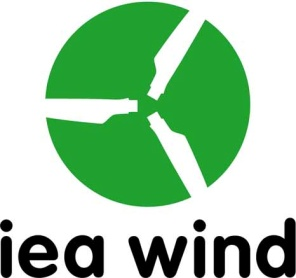
\includegraphics[height=2cm]{graphics/IEAWind_logo.jpg}  &
			The International Energy Agency is an autonomous organisation which works to ensure reliable, affordable and clean energy for its 30 member countries and beyond. The IEA Wind Technology Collaboration Programme supports the work of 38 independent, international groups of experts that enable governments and industries from around the world to lead programmes and projects on a wide range of energy technologies and related issues.%
			\\
			% Task 32 * DO NOT EDIT THIS TEXT *
			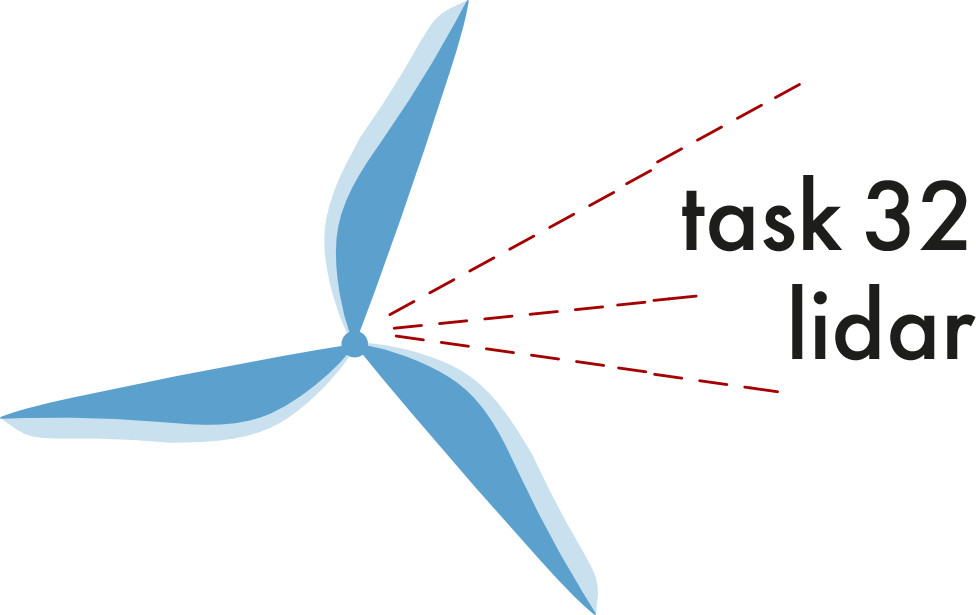
\includegraphics[height=1.5cm]{graphics/Task32_logo.jpg} &
			\href{https://community.ieawind.org/task32/home}{IEA Wind Task 32} exists to identify and mitigate the barriers to the deployment of wind lidar for wind energy applications.
		\end{tabular}%

		%% -----------------------------------
		%% For more information
		%% -----------------------------------
		% N.B. do not add line breaks between the next items
		\textbf{For more information:} See the  \href{https://community.ieawind.org/task32/home}{Task 32 website}.
		%% -----------------------------------
		%% Authors
		%% -----------------------------------
		\textbf{Author team:} %
		Andrew Clifton (Task 32 Operating Agent, University of Stuttgart, Germany), %
		David Schlipf (Task 32 operating Agent, Flensburg University of Applied Sciences, Germany).
		%% -----------------------------------
		%% Reviewers
		%% -----------------------------------
		%\textbf{Reviewers:} %
		% first last (short affiliation), %
		% first last (short affiliation).
		%% -----------------------------------
		%% Images
		%% -----------------------------------
		\textbf{Images:}
		Banner, left to right: \href{https://unsplash.com/@alexkixa}{Alexandre Debiève on Unsplash}, \href{http://ifb.uni-stuttgart.de}{SWE U. Stuttgart}, \href{https://unsplash.com/@markusspiske}{Markus Spiske on Unsplash}.
	}

	%% -----------------------------------
	%% End of highlighted block
	%% -----------------------------------
\end{tcolorbox}
\vspace*{\fill}

\end{document}
